   	\newpage
   	\section{Personas und Anwendungsszenarien}
   	Dieses Kapitel befasst sich mit Personas und deren Anwendungsszenarien. Eine Persona ist eine Person, die eine Gruppe von zukünftigen Nutzern der Applikation beispielhaft repräsentiert. Personas haben konkrete Eigenschaften und zeigen in einem Anwendungsszenario, wie sie mit dem Produkt umgehen wollen.
   	
	\subsection{Persona 1 - ,,Der Kontrollfreak'': Elisa Schubert (20)}
	\begin{center}
		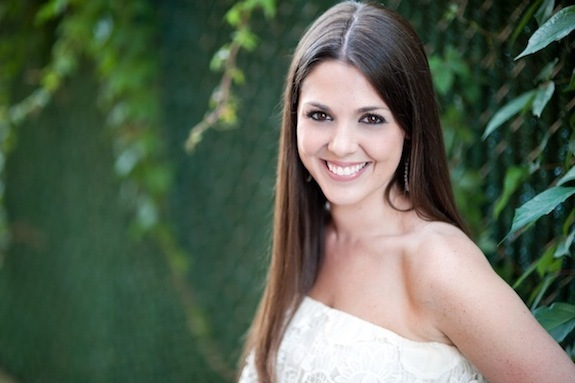
\includegraphics[width=0.7\textwidth]{persona_01.jpg}
	\end{center}
	\subsubsection{Soziodemografische Daten}
	Elisa Schubert ist 20 Jahre alt. Sie ist ledig und zur Zeit in einer festen Beziehung. Vor einem Jahr hat sie ihr Abitur gemacht. Aktuell studiert sie die Fächer Deutsch und Biologie an der Universität zu Köln.
	\subsubsection{Vorlieben, Hobbys, Abneigungen}
	Frau Schubert singt in einem Gospel-Chor, geht gern auf Partys und engagiert sich in ihrer Freizeit ehrenamtlich bei der Naturschutzorganisation WWF. Sie ist notorisch eifersüchtig auf jede Frau, die sich Ihrer Jugendliebe Bernd nähert. Da Bernd auch dafür bekannt ist, ,,mehrgleisig'' unterwegs zu sein, will sie immer wieder Gewissheit, dass er nur sie liebt. Frau Schubert hasst es belogen zu werden. Sie ist ein Kontrollfreak und liest heimlich die SMS von Bernd. Für ihre Zukunft hat sich Elisa vorgenommen, mit Bernd eine Familie gründen und Ihr Studium erfolgreich zu beenden. 
	\subsubsection{Nutzererwartung an das Produkt}
	Elisa ist neugierig was andere Menschen, insbesondere ihre Freunde, über sie denken. Sie erwartet von der LIAR App, dass sie Bernd besser kontrollieren kann und erhofft sich Einblicke in die verborgene Gedankenwelt ihrer Freunde.
	\subsubsection{Anwendungsszenario}
	An einem gemütlichen Samstag Abend spielen Elisa, Bernd und einige Freunde Karten- und Gesellschaftsspiele. Elisa hat die LIAR App, samt den dazugehörenden Sensoren mitgebracht und stellt sie ihren Freunden vor. So ist sie in der Lage auf unauffällige Art und Weise Bernd Fragen zu stellen und seine Antworten auf den Wahrheitsgehalt hin zu überprüfen. Die anderen Freunde stellen einander ebenfalls Fragen und haben dabei viel Spaß.
   
   	\subsection{Persona 2 - ,,Der Wissenschaftler'': Frank Bollwerker (36)}
   	\begin{center}
		
\includegraphics[width=0.7\textwidth]{persona_02.jpg}
	\end{center}
	\subsubsection{Soziodemografische Daten}
	Frank Bollwerker ist 36 Jahre alt, verheiratet und zur Zeit noch kinderlos. Er hat sein Physikstudium abgeschlossen und arbeitet seit dieser Zeit als wissenschaftlicher Mitarbeiter im Studiengang Luft- und Raumfahrttechnik an der Universität Stuttgart.
	\subsubsection{Vorlieben, Hobbys, Abneigungen}
	Frank ist ein gewissenhafter Forscher, der seit einem halben Jahr nach einem passenden Thema für seine Doktorarbeit sucht. Er überlegt, ob er erweiterte Tests zur Auswahl der zukünftigen Raumfahrer entwickeln sollte, welche neben den kognitiven und körperlichen Aspekten auch den Wahrheitswert von Antworten auf Fragen untersucht. Frank spielt in seiner Freizeit Bowling und geht gerne Wandern.
	\subsubsection{Nutzererwartung an das Produkt}
	Herr Bollwerker erwartet ein Produkt, was höchsten wissenschaftlichen Ansprüchen gerecht wird. Er erhofft sich mit der LIAR App signifikante und eindeutige Aussagen zu den Antworten von zukünftigen Raumfahrern zu erhalten.
	\subsubsection{Anwendungsszenario}
	Während der Fahrt mit den öffentlichen Verkehrsmitteln zu Universität findet Herr Bollwerker die LIAR-App im Google Play Store und beliest sich zum Thema Lügendetektor. Er beschließt die App zu kaufen und auf Verwendbarkeit für seine wissenschaftliche Arbeit zu testen.
	
	\subsection{Persona 3 - ,,Der Angeber'': Jonas Keppler (29)}
	\begin{center}
		
\includegraphics[width=0.7\textwidth]{persona_03.jpg}
	\end{center}
	\subsubsection{Soziodemografische Daten}
	Jonas Keppler ist 29 Jahre alt und ledig. Eine feste Freundin hat nicht, da diese wie die Hemden wechselt. Er nach seinem Germanistikstudium eine Journalistenschule in Bonn besucht. Nebenbei hat er in einem kleinen Softwareunternehmen als Webentwickler gearbeitet um seinen monatlichen Ausgaben zu decken. Seit 6 Monaten arbeitet als Redakteur im Ressort "Digital" bei der Süddeutschen Zeitung in München.
	\subsubsection{Vorlieben, Hobbys, Abneigungen}
	Herr Keppler ist sehr interessiert an neuer Technik und coolen Apps, die er dann stolz während der Mittagspause all seinen Arbeitskollegen präsentiert. Er 	steht gern im Mittelpunkt. Jeden Donnerstag geht ins Kino und schaut sich die neuesten Filme in der Sneak Preview an. Er immmer der Erste, der etwas Neues ausprobiert. Jonas Keppler macht Yoga und achtet sehr auf seine Ernährung. Er kauft im Biomarkt ein und wird im nächsten Sommer erstmals selbst Gemüse auf seinem Grundstück anbauen.
	\subsubsection{Nutzererwartung an das Produkt}
	Jonas erwartet ein Produkt, was sich als Publikumsmagnet für die nächste WG-Party eignet. Es muss andere Leute neugierig machen und sollte ihn als Entertainer dastehen lassen. 
	\subsubsection{Anwendungsszenario}
	Jonas Keppler im Internet von der LIAR-App gelesen und war der Erste, der sich den Prototyp bestellt hat. Den nächsten Werktag kann er gar nicht mehr abwarten, denn er weiß, dass ihm die Aufmerksamkeit der Kollegen damit gewiss ist.
